\documentclass[aps,10pt,a4paper]{article}

\usepackage{graphics}
\usepackage{graphicx}
\usepackage{graphics}
\usepackage{fancyvrb,enumerate}
\usepackage{amsmath,amssymb,amscd,amsfonts}
\usepackage{geometry}
\usepackage{multirow}
\usepackage{url}
\DeclareGraphicsExtensions{.pdf,.png,.jpg}

\geometry {
	paper=a4paper,
	top=20mm,
	bottom=20mm,
	left=25mm,
	right=25mm
}

\title{Inspection of MERS in the Clinical Point}
\author{Jaewoong Lee}
\date{2018.06.15.}

\begin{document}
	\maketitle
	\newpage
	
	\tableofcontents
	\listoftables
	\listoffigures
	\newpage
	
	\section{Introduction}
		\subsection{Coronavirus}
			Coronavirus, also know as CoV, is discovered in 1960s from patients with common cold, and these viruses were named human CoV 229E and OC43.\cite{ref:cold} Coronaviruses cause a significant percentage of common colds in human. Coronavirus OC43 or 229E infection was detected in 17 of the 200 patients.\cite{ref:rateCold} Common human coronaviruses usually cause mild to moderate upper-respiratory tract illnesses, however, some mutations of coronaviruses, for example SARS-CoV and MERS-CoV, have been known to frequently cause sever symptoms.\cite{ref:CoVCDC}
		
		\subsection{MERS Coronavirus}
			MERS, also known as Middle East respiratory syndrome, is a viral respiratory infection caused by the MERS-CoV, but it may be an overestimate of the true mortality rate.\cite{ref:MersWho} MERS-CoV causes many symptoms such as muscle pain, shortness or breath, and fever. Approximately 35\% of reported patients with MERS have died.\cite{ref:MersWho} MERS-Cov is derived from common CoV, but the fatality is significantly higher than common CoV, so we will find out the reason.
	
	\section{Object}
		\subsection{How MERS-CoV can be detected?}
			As I mentioned later, ORF 1ab is used for screening MERS-CoV. The set of coronavirus are too big, so there are no appropriate strategy to divide with common cold and MERS-CoV. Hence, in this inspection, we divide coronavirus set with scoring about ORF. 
	
		\subsection{How MERS-CoV avoid the antibody?}
			As I mentioned later, DPP4 affects to immune regulation. We assume that MERS-CoV has DPP4 somehow, so they can avoid immune response, and they have high fatality. 
	
	\section{Material}
		\subsection{ORF 1ab}
			ORF, also known as open reading frame, is the part of a reading frame that has ability to be translated. So an ORF is a continuous stretch of codons that contain a start codon and a stop codon. 
			Also, ORF 1ab is used for detection MERS CoV with real-time reverse-transcription polymerase chain reaction.\cite{ref:detectMERS}
		
		\subsection{DPP4}
			DPP4, also known as dipeptidyl peptidase-4 or CD26, is a protein that is encoded by the DPP4 gene. The protein encoded by the DPP4 gene is an antigenic enzyme expressed on the surface of most cell types and is associated with immune regulation, signal transduction and apoptosis. 
	
	\section{Method}
		\subsection{Sequence Alignment}
			A sequence alignment is a way of arranging the sequences of DNA, RNA, or protein to identify regions of similarity that may be a consequence of functional, structural, or evolutionary relationships between the sequences. Aligned sequences of nucleotide or amino acid residues are typically represented as row within a matrix. Gaps inserted between the residues so that identical or similar characters are aligned in successive columns.
			
			\subsubsection{Global Alignments \& Local Alignments}
				Global alignments, which attempt to align every residue in every sequence, are most useful when the sequence in the query set are roughly equal size. However, local alignments are more useful for dissimilar sequences that are suspected to contain regions of similar sequence motifs within their larger sequence context. In this inspection, I need to check that one sequence contains the other, so I used a local alignments only. 
				
			\subsubsection{BLOSUM}
				BLOSUM, which stands for blocks substitution matrix, is a substitution matrix used for sequence alignment of proteins. Also, scoring matrix is a matrix which describes the probability of a biological meaningful amino acid residue pair occurring in an alignment. BLOSUM matrices with high number are designed for comparing closely related sequences, while those with low numbers are designed for comparing distant related sequences. In this inspection, I used the BLOSUM50 and BLOSUM62. 
		
		\subsection{PyPy}
			\begin{figure}[htbp]
				\centering
				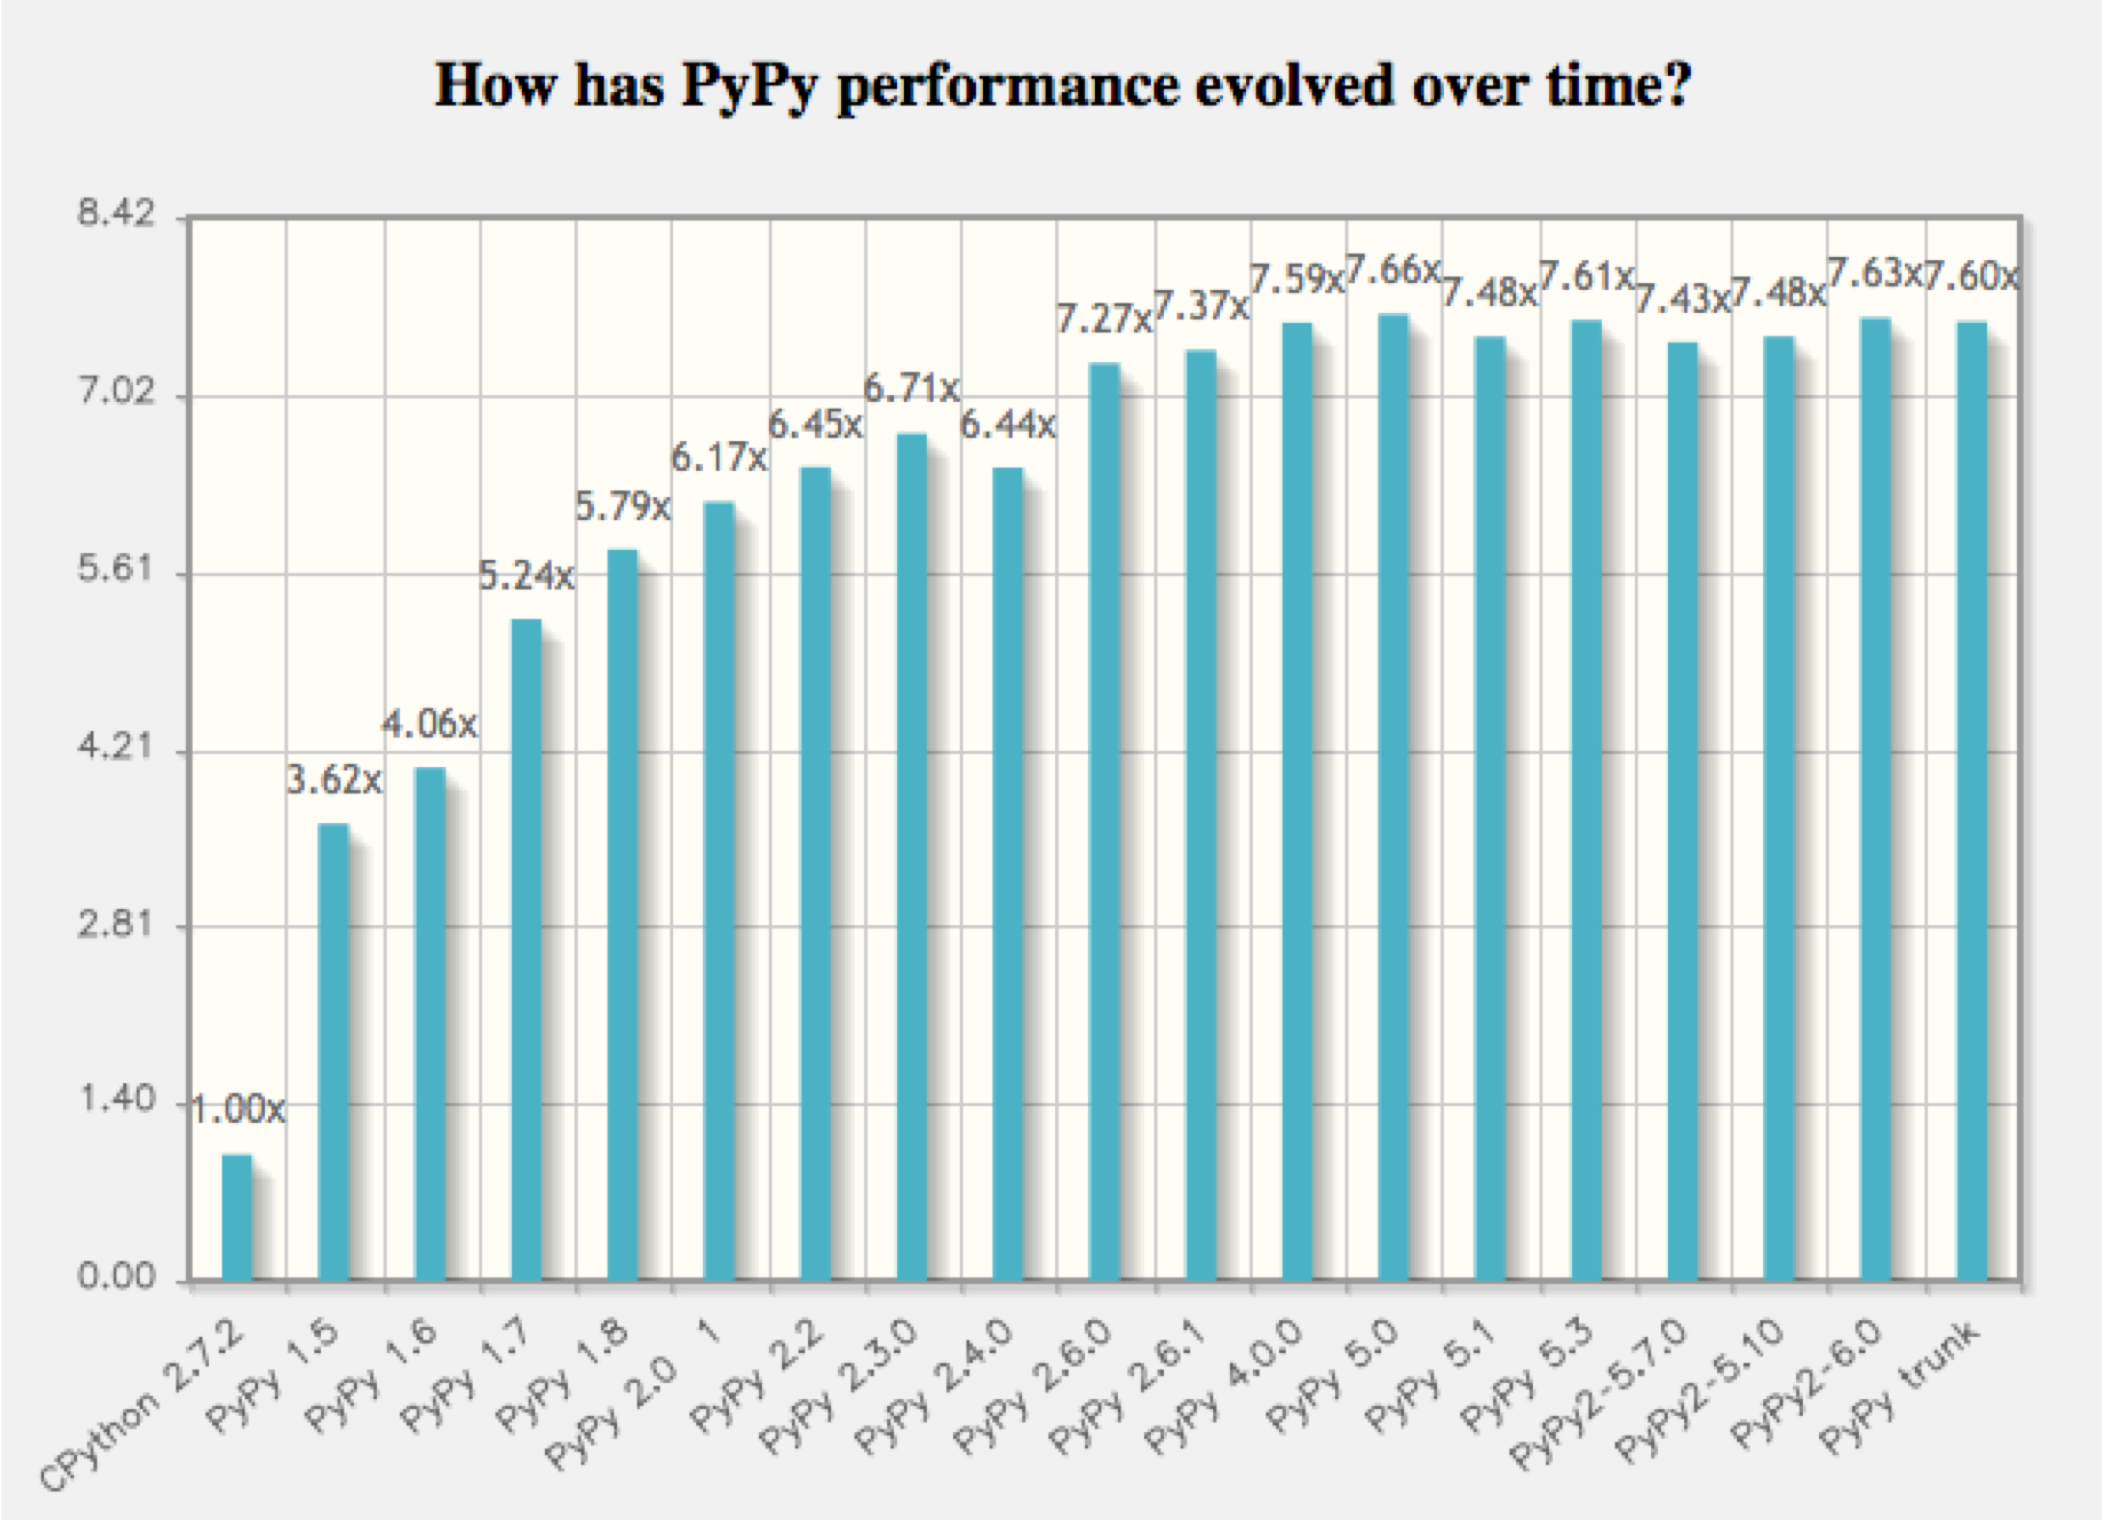
\includegraphics[height=6cm]{pypy}
				\caption{Speed Improvement of PyPy}
				\label{fg:pypy}
			\end{figure}
			PyPy is an alternative implementation of the Python which often runs faster than the standard implementation of Python. PyPy is a just-in-time compiler while CPython, the standard, is an interpreter, so PyPy is faster than CPython. The speed improvement of PyPy is as shown as the figure \ref{fg:pypy}.
	
	\newpage
	\section{Result}
		\subsection{ORF with BLOSUM50}
			The local alignment score of ORF with BLOSUM50 is shown as the table \ref{tb:orf50}. Also, the graph which from the table \ref{tb:orf50} is the graph \ref{fg:orf50}. 
			\begin{table}[h!]
				\centering
				\caption{Local Alignment Score of ORF with BLOSUM62}
				\label{tb:orf50}
				\begin{tabular}{ c || c | c }
					& Average & Standard Deviation \\ \hline
					All & 75.56527415 & 7.41806982 \\
					MERS & 83 & 4.359748549 \\ 
					SARS & 73.95859873 & 6.960462913 \\
				\end{tabular}
			\end{table}
		
			\begin{figure}[htbp]
				\centering
				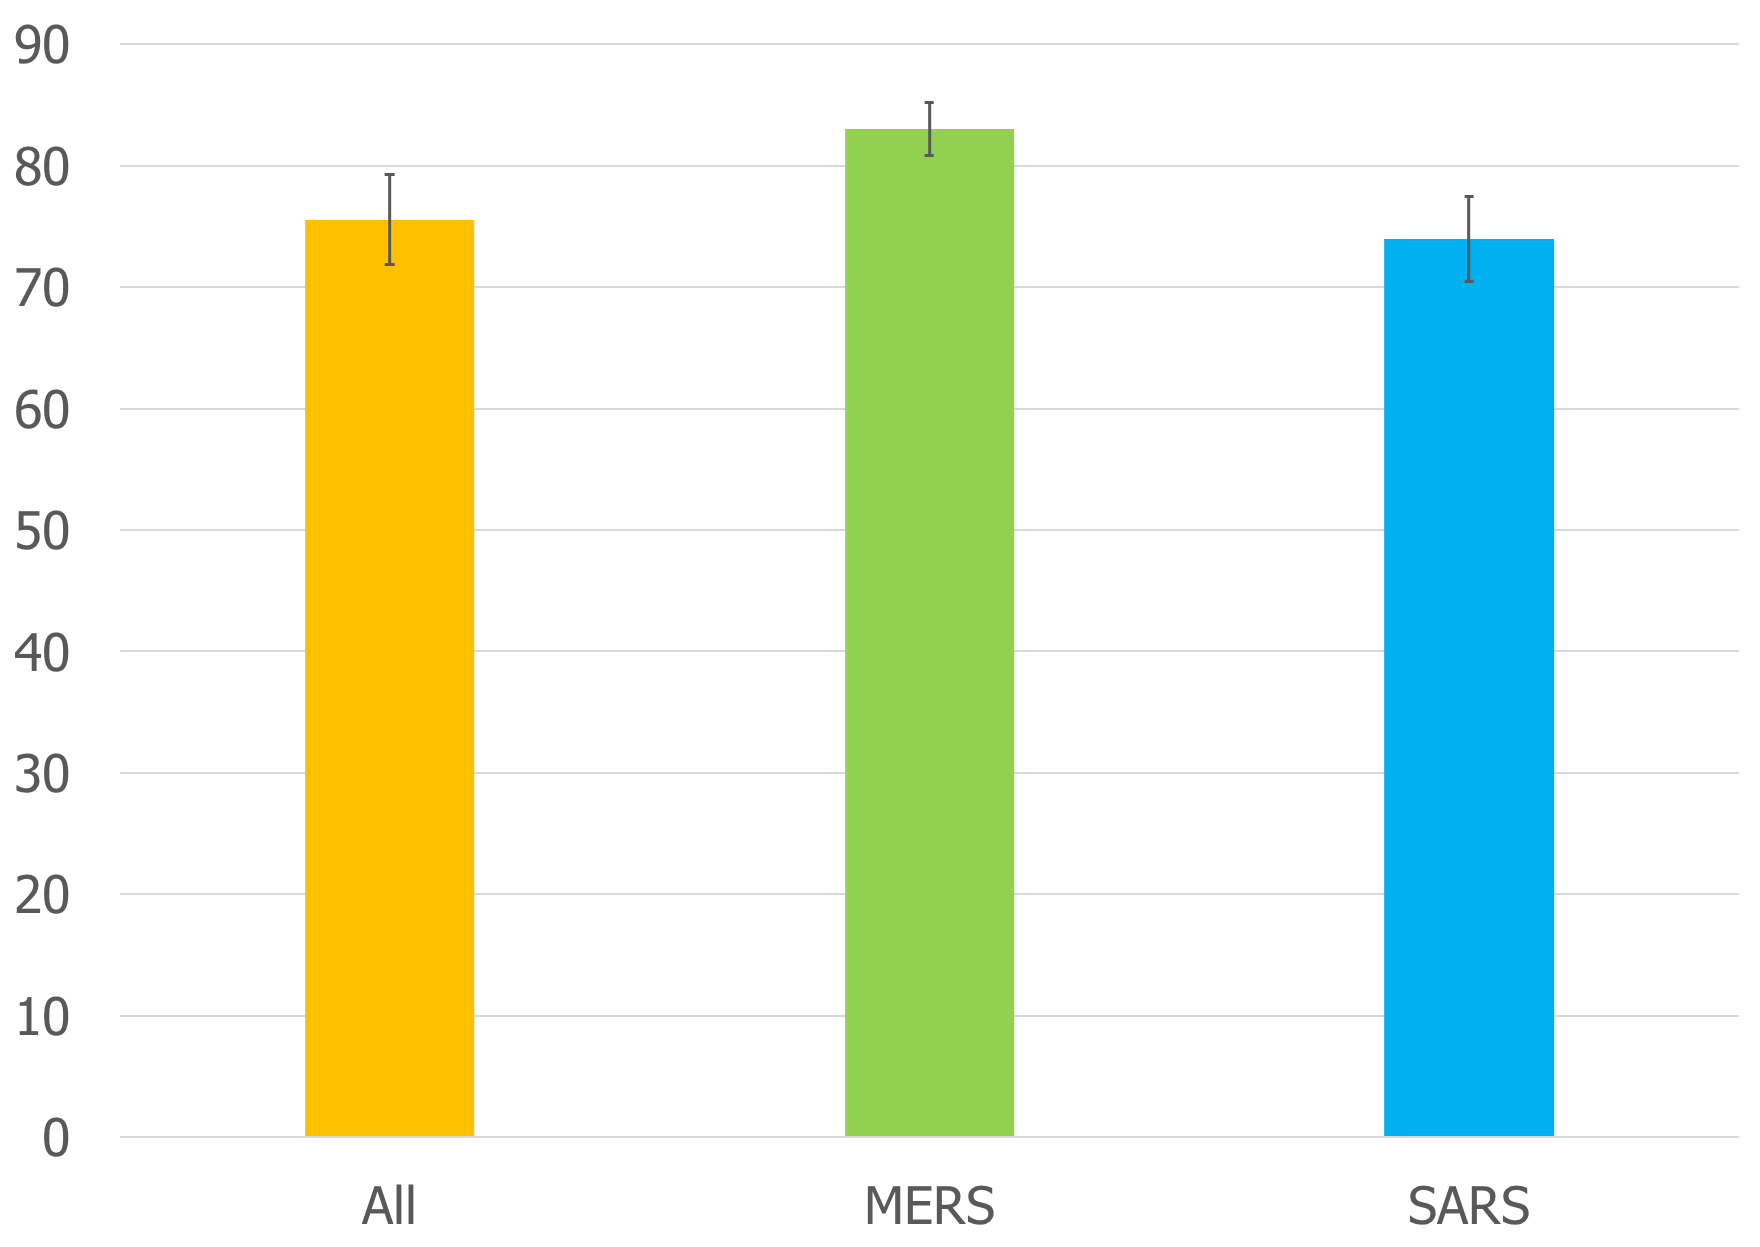
\includegraphics[height=5cm]{ORF50}
				\caption{Local Alignment Score of ORF with BLOSUM50}
				\label{fg:orf50}
			\end{figure}
		
		\subsection{ORF with BLOSUM62}
			The local alignment score of ORF with BLOSUM62 is shown as the table \ref{tb:orf62}. Also, the graph which from the table \ref{tb:orf62} is the graph \ref{fg:orf62}. 
			\begin{table}[h!]
				\centering
				\caption{Local Alignment Score of ORF with BLOSUM62}
				\label{tb:orf62}
				\begin{tabular}{ c || c | c }
					& Average & Standard Deviation \\ \hline
					All & 48.47650131 & 3.999522361 \\
					MERS & 50.97794118 & 1.057368584 \\ 
					SARS & 47.92993631 & 4.196702054 \\
				\end{tabular}
			\end{table}
		
			\begin{figure}[htbp]
				\centering
				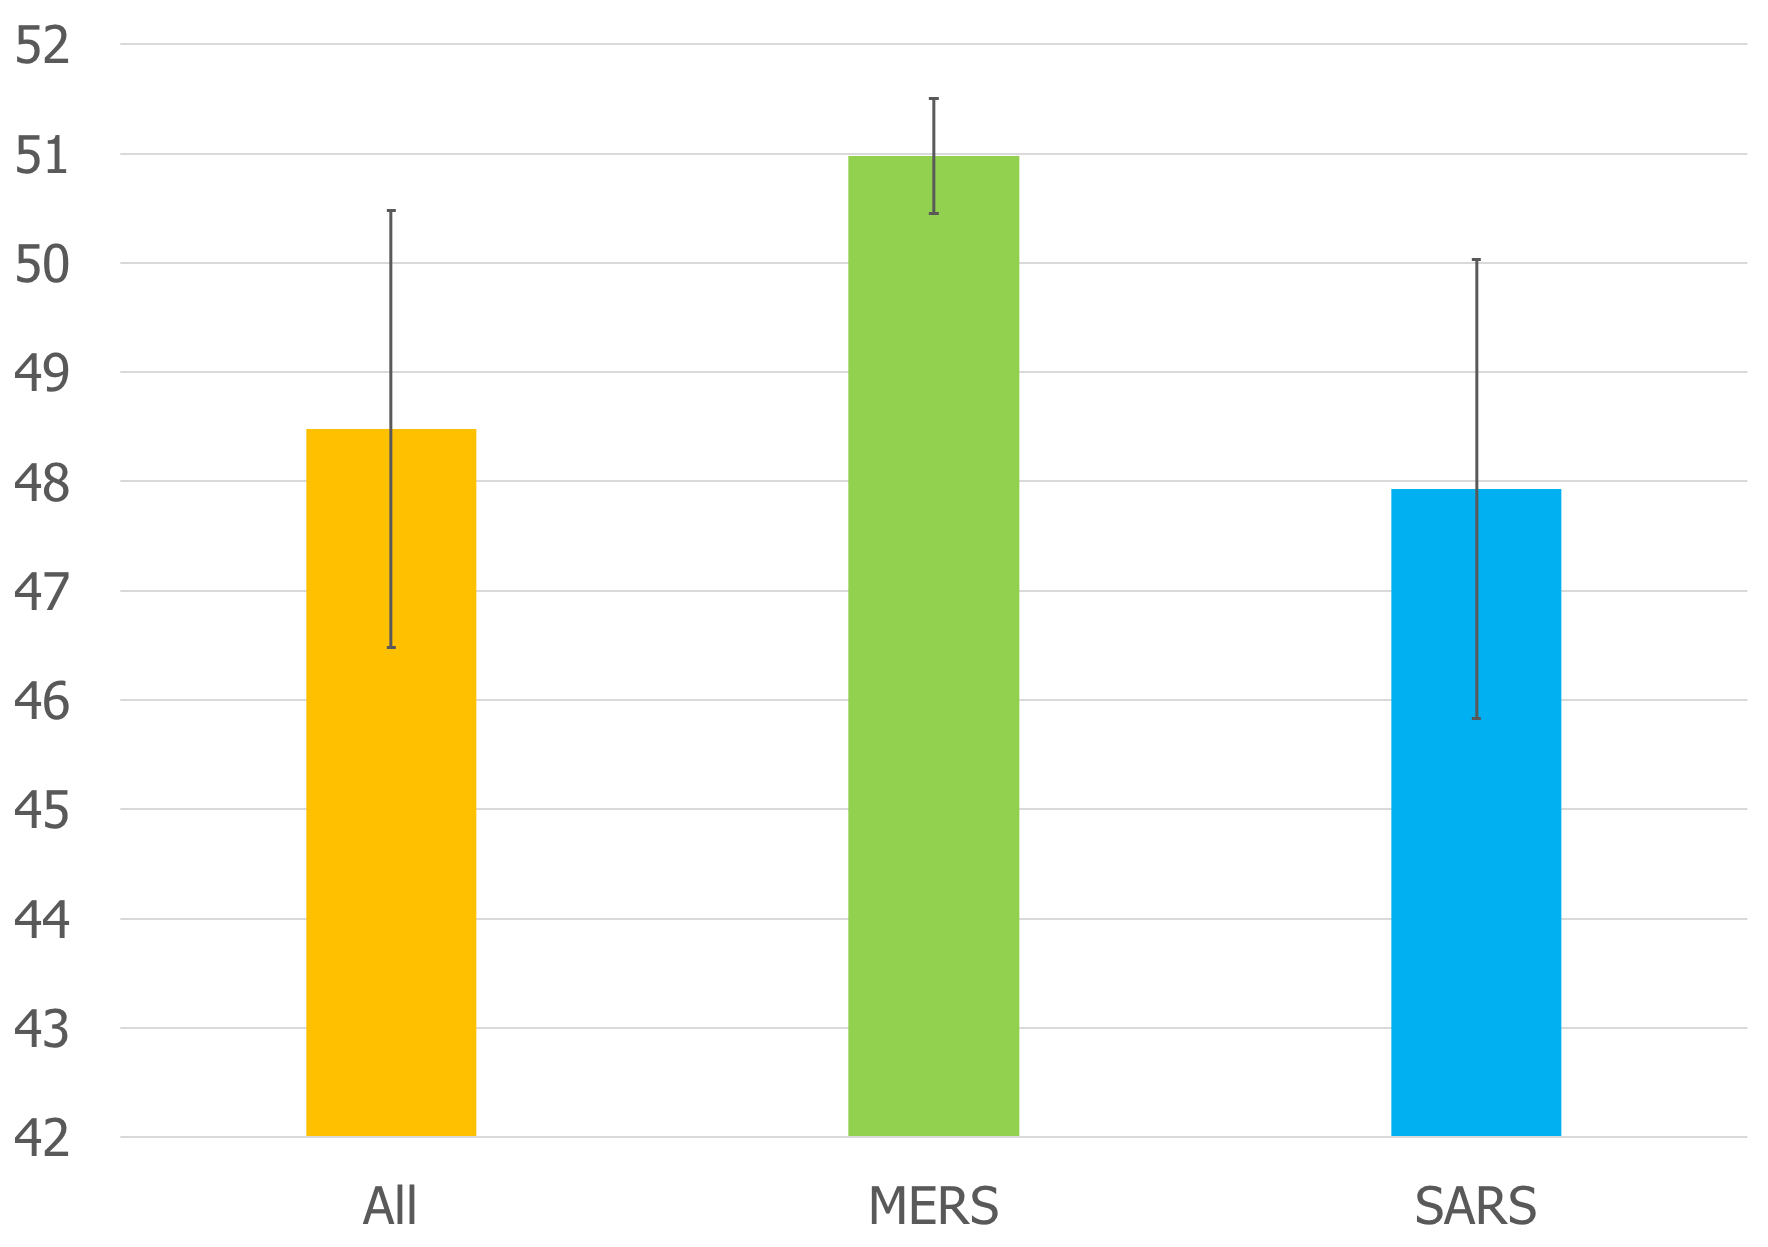
\includegraphics[height=5cm]{ORF62}
				\caption{Local Alignment Score of ORF with BLOSUM62}
				\label{fg:orf62}
			\end{figure}
		
		\subsection{DPP4 with BLOSUM50}
			The local alignment score of DPP4 with BLOSUM50 is shown as the table \ref{tb:dpp450}. Also, the graph which from the table \ref{tb:dpp450} is the graph \ref{fg:dpp450}. 
			\begin{table}[h!]
				\centering
				\caption{Local Alignment Score of DPP4 with BLOSUM50}
				\label{tb:dpp450}
				\begin{tabular}{ c || c | c }
					& Average & Standard Deviation \\ \hline
					All & 66.9843342 & 6.744236175 \\
					MERS & 63.77941176 & 3.882899216 \\
					SARS & 67.65605096 & 7.014874491 \\
				\end{tabular}
			\end{table}
	
			\begin{figure}[htbp]
				\centering
				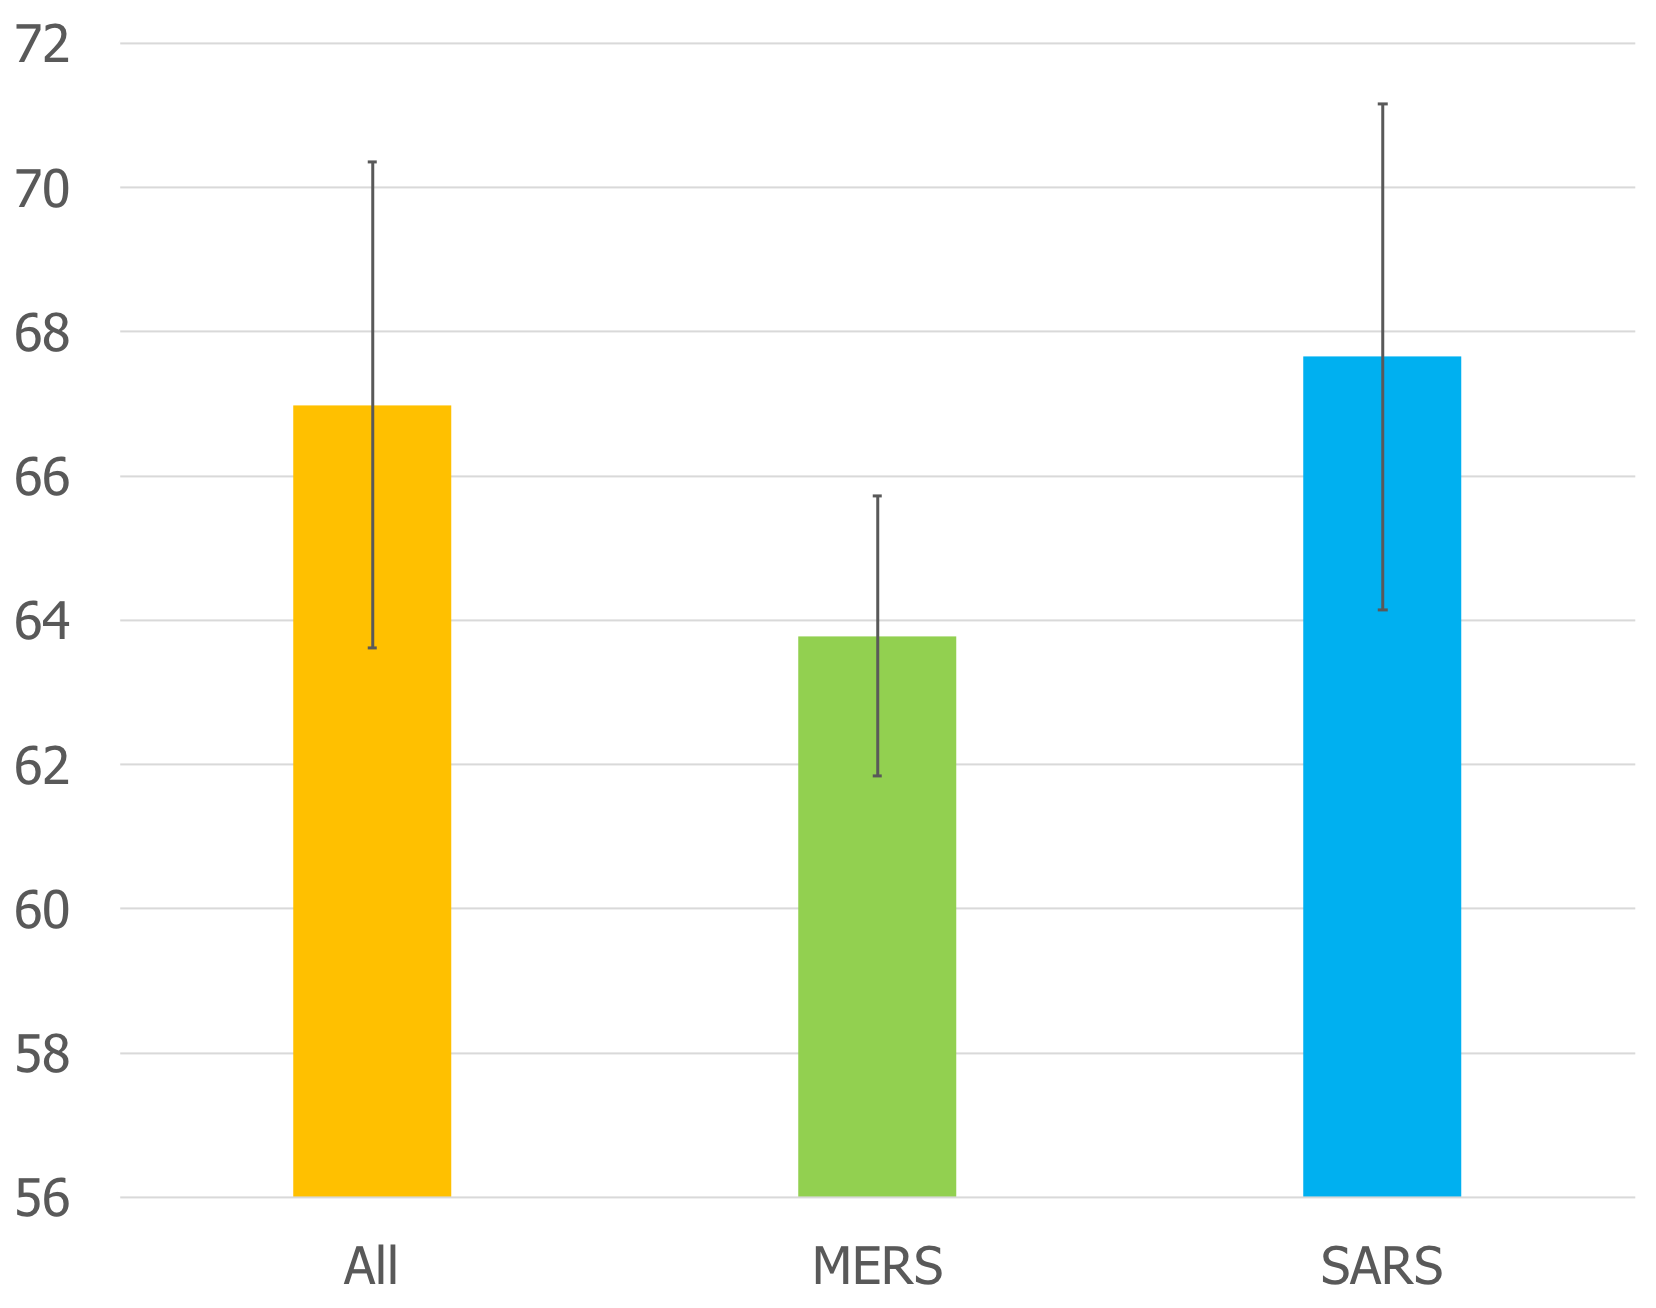
\includegraphics[height=5cm]{DPP450}
				\caption{Local Alignment Score of DPP4 with BLOSUM50}
				\label{fg:dpp450}
			\end{figure}
		
		\subsection{DPP4 with BLOSUM62}
			The local alignment score of DPP4 with BLOSUM62 is shown as the table \ref{tb:dpp462}. Also, the graph which from the table \ref{tb:dpp462} is the graph \ref{fg:dpp462}. 
			\begin{table}[h!]
				\centering
				\caption{Local Alignment Score of DPP4 with BLOSUM62}
				\label{tb:dpp462}
				\begin{tabular}{ c || c | c }
					& Average & Standard Deviation \\ \hline
					All & 42.81201044 & 4.363683984 \\
					MERS & 44.93382353 & 1.055512555 \\ 
					SARS & 67.65605096 & 7.014874491 \\
				\end{tabular}
			\end{table}
		
			\begin{figure}[htbp]
				\centering
				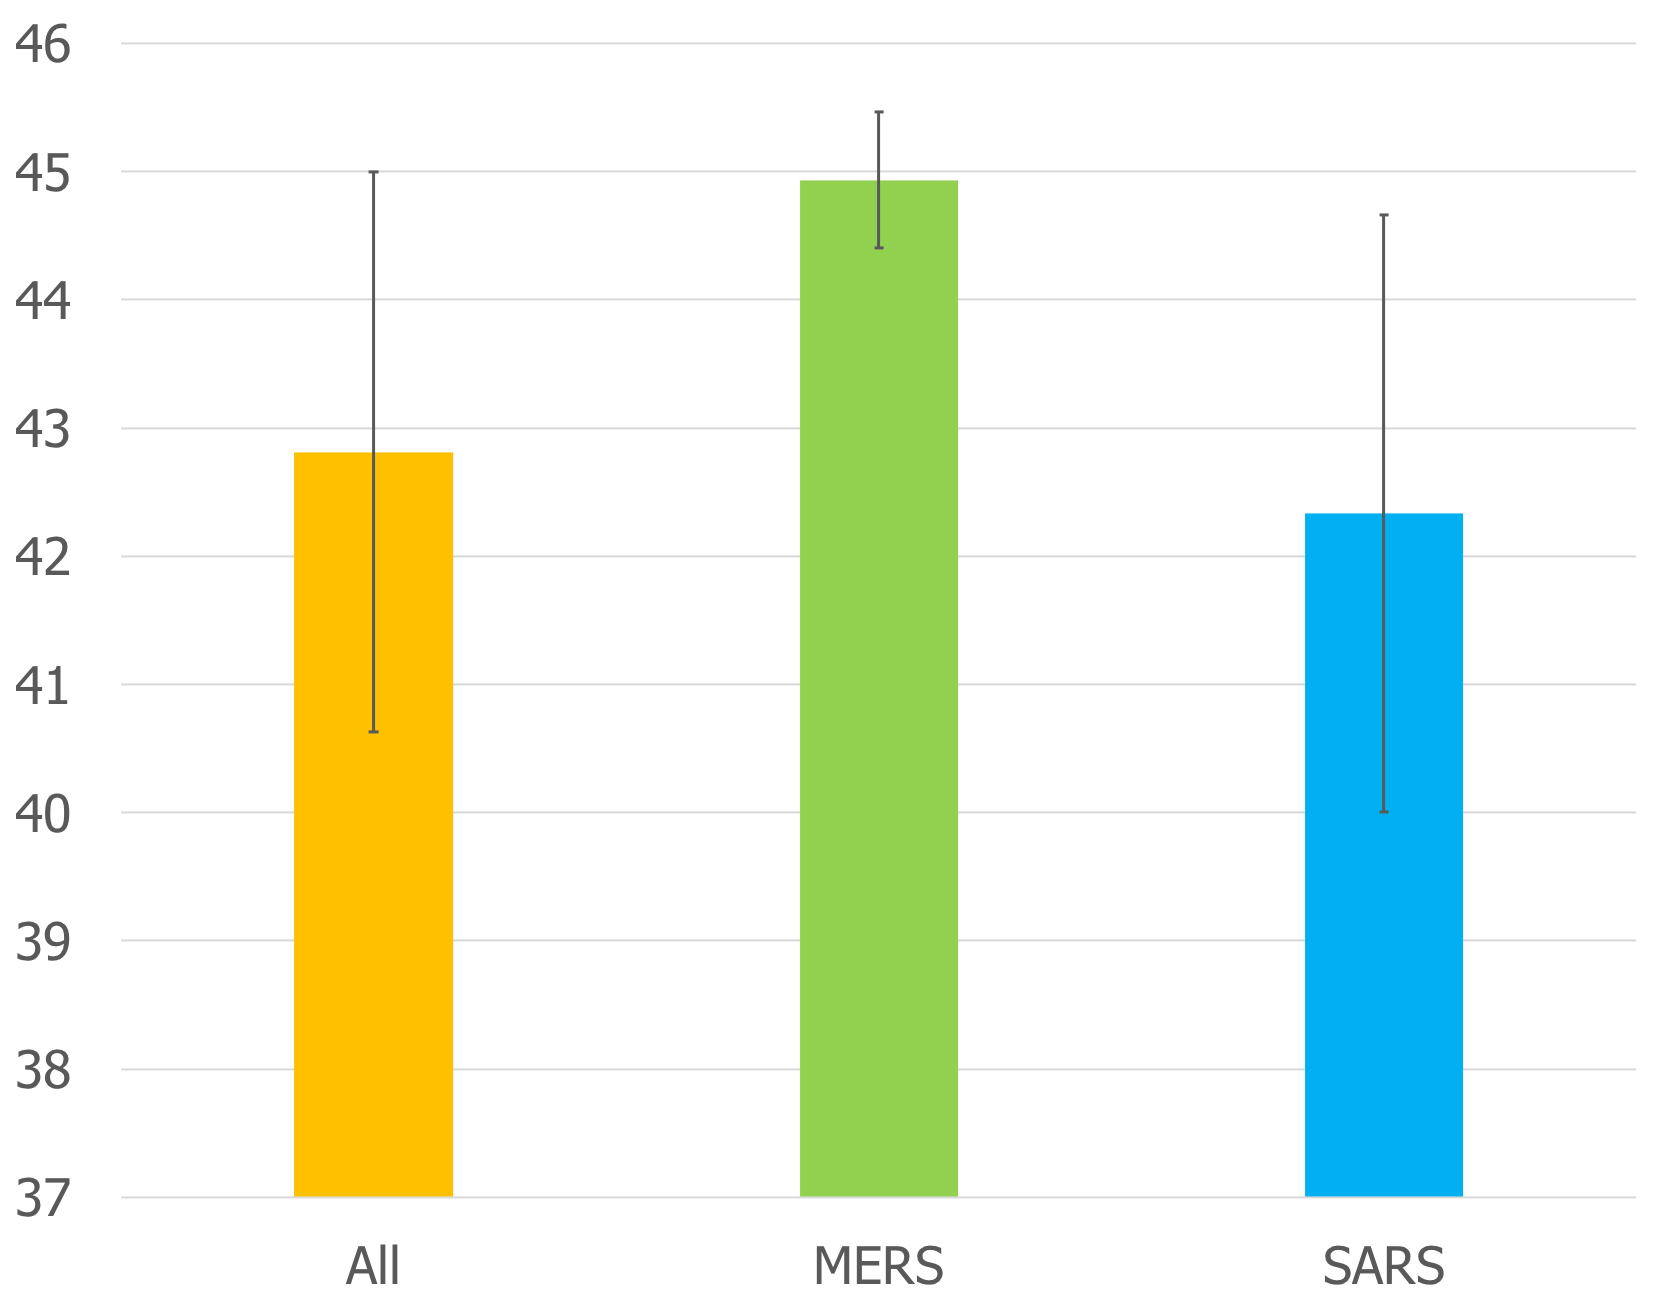
\includegraphics[height=5cm]{DPP462}
				\caption{Local Alignment Score of DPP4 with BLOSUM62}
				\label{fg:dpp462}
			\end{figure}
	
	\section{Discussion}
		\subsection{ORF}
			As comparing the figure \ref{fg:orf50} and the figure \ref{fg:orf62}, they have similar appearance. As I mentioned hereinabove, ORF is used for screening MERS-CoV, so there should be sub-sequence of MERS-CoV which is similar to ORF. Hence, MERS-CoV has higher score than other group.
		
		\subsection{DPP4}
			In the figure \ref{fg:dpp450}, MERS-CoV has lower score than the other; however, in the figure \ref{fg:dpp462}, MERS-CoV has higher score than the other. The DPP4-similar region of MERS-CoV is came from host, in other word, MERS-CoV copied from host. Hence, there should be sub-sequence of MERS-CoV which is almost identical, over similar, to DPP4, so the score with BLOSUM50 is lower than with BLOSUM62.
		
	\section{Suggestion}
		\subsection{Gene Set}
			In this inspection, we used some kind of coronavirus; common cold CoV, MERS-CoV, and SARS-CoV. However, the size of common cold CoV is only two, so we cannot calculate the statistics value. 
		
		\subsection{Wobble}
			The given gene represented with DNA sequence, not amino acid sequence. So, in this inspection, I translate DNA sequence into amino acid sequence as cell does. Also, in DNA sequence, there are some wobbles, but I randomly choose what they translate into. For example, W can be A and T, but I assume that W only can be A. In the next research, I want to make the program to choose really random, and repeats that many times, then it can be more closer to real nature.
		
		\subsection{BLOSUM}
			 In this inspection, I calculated sequence alignment with BLOSUM50 and BLOSUM62. If I do this inspection with more BLOSUM matrix, then I can confirm that my analysis is more exactly or not. 
	
	\bibliographystyle{unsrt}
	\bibliography{reference}
\end{document}